%% LyX 2.4.4 created this file.  For more info, see https://www.lyx.org/.
%% Do not edit unless you really know what you are doing.
\documentclass[english]{article}
\usepackage[T1]{fontenc}
\usepackage[latin9]{inputenc}
\usepackage{units}
\usepackage{enumitem}
\usepackage{amsmath}
\usepackage{amsthm}
\usepackage{cancel}
\usepackage{geometry}
\geometry{verbose,tmargin=1in,bmargin=1in,lmargin=1in,rmargin=1in}

\makeatletter

%%%%%%%%%%%%%%%%%%%%%%%%%%%%%% LyX specific LaTeX commands.
%% Because html converters don't know tabularnewline
\providecommand{\tabularnewline}{\\}

%%%%%%%%%%%%%%%%%%%%%%%%%%%%%% Textclass specific LaTeX commands.
\numberwithin{equation}{section}
\numberwithin{figure}{section}
\newlength{\lyxlabelwidth}      % auxiliary length 

%%%%%%%%%%%%%%%%%%%%%%%%%%%%%% User specified LaTeX commands.
\usepackage{hyperref}
\usepackage[usenames,dvipsnames,table]{xcolor} %adds additional color options
\hypersetup{colorlinks=true, urlcolor=black,linkcolor=black}

\usepackage{fancyhdr}
\usepackage{lastpage}
\pagestyle{fancy}
\usepackage{enumitem}
\usepackage{ifthen}
%sets math fonts to be more readable
\everymath=\expandafter{\the\everymath\displaystyle}
%\DeclareMathSizes{10}{10}{10}{10}
\usepackage{multicol}

\usepackage{tikz}
\usetikzlibrary{plotmarks}
\usepackage{pgfplots}
\pgfplotsset{compat=newest}

\usepackage{calc}
\usepackage[nomessages]{fp}

\usepackage{advdate}    % Advancing/saving dates
\usepackage{datetime}   % Dates formatting
\usepackage{datenumber} % Counters for dates

\usepackage{fancybox} %%ovalbox and fancy box settings

\usepackage[super]{nth} %easy 1st, 2nd, etc

\usepackage{forest} %%for tree diagram
% Added by lyx2lyx
\setlength{\parskip}{\smallskipamount}
\setlength{\parindent}{0pt}

\makeatother

\usepackage{babel}
\begin{document}
\renewcommand{\author}{Dr.\,James Ashe}

\newcommand{\classNum}{107}

\newcommand{\classSec}{7 and 10}

\newcommand{\nameType}{Name:}

\newcommand{\examType}{Exam 3}

\renewcommand{\date}{\formatdate{27}{10}{2014}}

%%First page's header%%%%%%%%%%%%%%%%%%%%%%
\fancypagestyle{firststyle} %%header settings for first pagr
{
	\fancyhead[L]{MTH \classNum{}(\classSec{}) \author{}\\
	\textbf{\examType{}} \date{}}
	\fancyhead[C]{\textbf{\nameType}}
	\setlength{\headsep}{14pt}
}
%%%%%%%%%%%%%%%%%%%%%%%%%%%%%%%%%%%%%%%%%%

%%Next page's header%%%%%%%%%%%%%%%%%%%%%%%
%\setlist{nolistsep}
\lhead{MTH \classNum{}(\classSec{})} 
\chead{\textbf{\nameType}} 
\cfoot{\thepage{}~of~\pageref{LastPage}} 
\setlength{\headsep}{5pt} 
%%%%%%%%%%%%%%%%%%%%%%%%%%%%%%%%%%%%%%%%%%%

%%Various settings; see the preamble for other settings%%%%%
%%\setenumerate[0]{leftmargin=12pt,itemindent=0pt,labelwidth=0pt}
%\setlist[2]{noitemsep}
%\setlist{nosep}
\setlist{itemsep=-3pt,topsep=-2pt}
\renewcommand{\labelenumi}{\textbf{\arabic{enumi}.}}
\renewcommand{\labelenumii}{\textbf{\alph{enumii}.}}
\thispagestyle{firststyle}
%%%%%%%%%%%%%%%%%%%%%%%%%%%%%%%%%%%%%%%%%%
\newcommand{\xmax}{10}
\newcommand{\xmin}{-10}
\newcommand{\xstep}{0} %must be xmin+n
\newcommand{\ymax}{10}
\newcommand{\ymin}{-10}
\newcommand{\ystep}{0} %must be ymin+n

\newcommand{\xspace}{\hspace*{40pt}}
\newcommand{\yspace}{\vspace*{1.4cm}}
\newcommand{\rowColor}{gray!35}
\large

\emph{Unless stated otherwise, all problems are worth 3 points and
answers should be stated as exact fractions or decimals rounded to
three decimal places. You must show your work to receive credit. }
\begin{enumerate}[resume]
\item A card is dealt from a well-shuffled, standard deck of $52$ cards.
Find the probability of being dealt each of the following (write your
answer as a fraction).\begin{multicols}{2}

\begin{enumerate}
\item an ace\yspace\yspace
\item the ace of spades\yspace\yspace
\item an ace or a spade\yspace\yspace
\item A four of spades\yspace\yspace
\end{enumerate}
\end{multicols}\vfill
\item A coins is flipped and a six-sided die is tossed. Find the following:\begin{multicols}{2}

\begin{enumerate}
\item the sample space\\
\yspace\columnbreak
\item the probability of getting a head AND rolling a three. \yspace\yspace
\item {[}2 points{]} the odds of getting a head AND rolling a three.\yspace
\item the probability of getting a head OR rolling a three.\yspace\yspace
\item {[}2 points{]} the odds of getting a head OR rolling a three. \yspace
\end{enumerate}
\end{multicols}\vfill\newpage
\item {[}6 points each{]} Complete the following:

\begin{enumerate}
\item The MHU librarian has found that the number of books checked out by
students is as follows:

\begin{enumerate}
\item []%
\begin{tabular}{|c|c|c|c|c|}
\hline 
\textbf{Number of Books} & 0 & 1 & 2 & 3\tabularnewline
\hline 
\textbf{proportion} & 25\% & 50\% & 15\% & 10\%\tabularnewline
\hline 
\end{tabular}
\end{enumerate}
Find the expected number of books checked out by a student.\yspace\yspace
\item You have been asked to play a game with a six-sided die. The rules
are as follows.

\begin{itemize}
\item If you roll a 1 or 2 you win \$50.
\item If you roll a 3 you lose \$10.
\item If you roll a 4, 5, or 6 you lose \$20
\end{itemize}
Find the expected value of the game. \yspace\yspace\vfill
\end{enumerate}
\item Approximately 66\% of the cars at Big Bill's Cars are new and 34\%
are used. Of the new cars, 75\% are Fords and the rest are Hondas.
While 40\% of the used cars are Fords and the rest are Hondas.\begin{multicols}{2}

\begin{enumerate}
\item Complete the tree diagram describing the probability\\
\tikzset{abovelabel/.style={midway,above,font=\scriptsize}} 
\tikzset{belowlabel/.style={midway,below,font=\scriptsize}} 

\forestset{  
	L1/.style={rectangle, rounded corners, very     thick},   	
	L2/.style={rectangle, rounded corners, very     thick,
		edge={black,line width=.75pt,line cap=round}},   	
	L3/.style={rectangle, rounded corners, very     thick,
		edge={black,line width=.75pt,line cap=round}},   	
	L4/.style={rectangle, rounded corners, very     thick,
	edge={black,line width=.75pt,line cap=round}}, 
}

\begin{forest}     
	for tree={
		scale=1,        
		grow=0,
		reversed, %tree direction         
		parent anchor=east,
		child anchor=west, %edge anchors   		edge={line cap=round},
		outer sep=+1pt, 
		%edge/node connection rounded corners,
		%minimum width=15mm,
		minimum height=15mm, 
		%node shape
		l sep=1.5cm    
		}   
[Start,L1
	[New,edge label={node[abovelabel,left=4pt]{\framebox{\vphantom{\huge HI} \hphantom{2555\%}}}},L2
		[Ford, edge label={node[abovelabel,above=4pt]{\framebox{\vphantom{\huge HI} \hphantom{2555\%}}}}, L3]         
		[Honda,edge label={node[belowlabel,below=4pt]{\framebox{\vphantom{\huge HI} \hphantom{2555\%}}}}, L3]               
	]
	[Used,edge label={node[belowlabel,left=4pt]{\framebox{\vphantom{\huge HI} \hphantom{2555\%}}}},L2
		[Ford, edge label={node[abovelabel,above=4pt]{\framebox{\vphantom{\huge HI} \hphantom{2555\%}}}}, L3]        
		[Honda,edge label={node[belowlabel,below=4pt]{\framebox{\vphantom{\huge HI} \hphantom{2555\%}}}}, L3]                
	]  
] 
\end{forest}\yspace\vfill\columnbreak
\item find the probability that a new car is a Ford.\yspace\yspace
\item find the probability that a car is new and a Ford.\yspace\yspace
\item find the probability that a car on the lot is a Ford. \yspace\yspace\vspace{-.6cm}
\end{enumerate}
\end{multicols}\vfill\newpage
\item Below are the results of a Gallup poll in which workers were asked
``Would you prefer a male or female boss?''

\begin{tabular}{|c|c|c|c|}
\hline 
 & \textbf{Prefer Male boss} & \textbf{Prefer Female boss} & \textbf{No preference}\tabularnewline
\hline 
Male & 29\% & 18\% & 53\%\tabularnewline
\hline 
Female & 40\% & 27\% & 33\%\tabularnewline
\hline 
\end{tabular}
\begin{enumerate}
\item What is the probability that a worker prefers a female boss?\yspace\yspace
\item What is the probability that a worker prefers a male boss given that
they are female?\yspace\yspace
\item What is the probability that someone is female given that they prefer
a male boss?\yspace\yspace
\end{enumerate}
\vfill
\item Of the students who are Biology majors, 55\% are taking Math, 65\%
are taking Art, and 30\% are taking both courses. Find the probability
of the following:\begin{multicols}{2}

\begin{enumerate}
\item a biology major is not taking Math\yspace\yspace
\item a biology major is taking Math or Art\yspace\yspace
\item a biology major is not taking Math and not taking Art. \yspace\columnbreak
\end{enumerate}
%%%% M or A %%%%%
\begin{center}
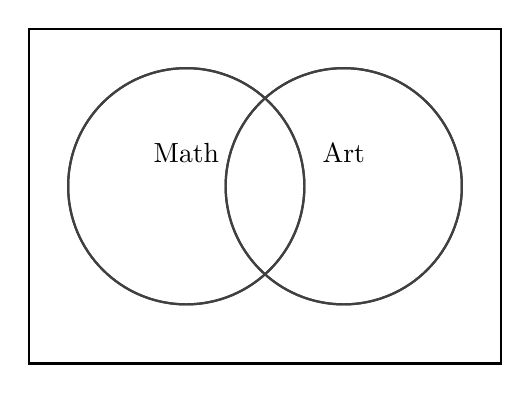
\begin{tikzpicture}[scale=1.0]
	\def\circleA{(0,0) circle (1.5)} %A
	\def\circleB{(0:2) circle (1.5)} %B

	\colorlet{circle edgeA}{black!75} 
	\colorlet{circle areaA}{red!100}
	\colorlet{circle edgeB}{black!75} 
	\colorlet{circle areaB}{green!100}

	\tikzset{
		filledA/.style={fill=circle areaA, draw=circle edgeA, thick},
		filledB/.style={fill=circle areaB, draw=circle edgeB, thick},
		outlineA/.style={draw=circle edgeA, thick},
		outlineB/.style={draw=circle edgeB, thick},
	}
	
	\begin{scope}[fill opacity=0.0]         
			\fill[filledA] \circleA;
			\fill[filledB] \circleB;    
	\end{scope}

	\draw[outlineA] \circleA node[above=5pt] {Math} node[] { $$} node[below=-1pt] at (0,-1.5) {$$}; 
	\draw[outlineB] \circleB node[above=5pt] {Art} node[] { $$} node[below=-1pt] at (2,-1.5) { $$};
	\draw (1,0) node {};
	\draw[thick] (-2,-2.25) rectangle (4,2) node[anchor=south east] at (current bounding box.south east) {$$}; 
\end{tikzpicture}
\end{center}

\end{multicols}\vfill\newpage
\item A die is rolled. The probability of rolling a 5 is $\nicefrac{1}{6}$,
and the probability of rolling a 5 given that a 4 or higher is rolled
is $\nicefrac{1}{3}$.\\
The probability of rolling a 4 or 5 is $\nicefrac{2}{6}=\nicefrac{1}{3}$,
and the probability of rolling a 4 or 5 given that an even number
is rolled is $\nicefrac{1}{3}$. Justify your answers.

\begin{enumerate}
\item Are the events ``rolling a 5'' and ``rolling a 4 or higher'' independent
or dependent?\yspace
\item Are the events ``rolling a 5'' and ``rolling a 4 or higher'' mutually
exclusive or non-mutually exclusive? \yspace
\item Are the events ``rolling a 5'' and ``rolling an even number''
mutually exclusive or non-mutually exclusive? \yspace
\item Are the events ``rolling a 4 or 5'' and ``rolling an even number''
independent or dependent?\yspace\vfill
\end{enumerate}
\item {[}6 points each{]} A jar contains 30 jellybeans. $12$ are red and
$18$ are blue. Jane randomly picks $5$ jellybeans. Find the probability
of each of the following. \textbf{You only need to write the formulas.}
\begin{multicols}{2}

\begin{enumerate}
\item all $5$ are blue.\yspace\yspace
\item exactly $4$ are blue.\yspace\yspace\columnbreak
\item $2$ red and $3$ blue. \yspace\yspace
\item at least $4$ are blue.\yspace\yspace
\end{enumerate}
\end{multicols}\vfill
\end{enumerate}
\newpage\vspace*{0cm}\vfill

\section*{Honor Statement}

\emph{On my honor, I have neither given nor received any academic
aid or information that would violate the Honor Code of Mars Hill
University.}\vspace{.5cm}
\begin{itemize}
\item []Signature:\underline{\hspace{7cm}}\vfill
\end{itemize}

\end{document}
